\section{Lezione 32 - 05/12/2023}

\subsection{MergeSort}
COPIA E INCOLLATO DA ALEX

Merge Sort, data un array di lunghezza $n$
idea: Se la lunghezza è sufficientemente grande (arbitrariamente >1), la decompongo in suddivisioni di grandezza 1 che è piu facile ordinare. La soluzione è imporatnte per lunghezza >1.
Prendo quindi l'elemento di mezzo dell'array e decompongo la seqeunz in 2 sottosequenze.

Separatamente ordino (con 2 chiamate ricorsive) le due sottosequenze.
Mi aspetto che le due sottoseuqenze siano internamente ordinate.
Le chiamate fanno ricorsivamente la stessa cosa dell'inizio. cioe vanno a suddividere le sequenze in sottosequenze ordinariamente piu piccole e a metà


Avere 2 sottosequenze ordinate non vuol dire che tutta la sequenza (unita) è ordinata.

A noi interessa dunque costruire la soluzione del problema principale, cioe ordinare completamente le due sottosequenze.

Problema suddiviso in 2 sottoprocedure:
- Decomposizione
- Ricomposizione delle due sottosequenze

\begin{lstlisting}[language=Java]
MergeSort(A,p,r) //A: Array, p: inizio, r: fine
    if p < r then:
        q=(p+r)/2 //prendiamo punto medio
        MergeSort(A,p,q) //chiamata ricorsiva sulla prima meta'
        MergeSort(A,q+1,r) //chiamata ricorsiva sulla seconda meta'
        Merge(A,p,q,r) //unione delle due meta' ordinate
\end{lstlisting}
Questo algoritmo funziona solo se vale la seguente condizione:
$$p \le q < r$$
Questo perché se non valesse ci sarebbe un loop infinito che non porterebbe a termine la compilazione.\bigskip

Esiste una versione più semplice che usa una struttura d'appoggio (Array), inserendo ogni volta l'elemento più piccolo tra i due insiemi, scartandolo poi quello che è stato inserito, seleziona i minimi delle due sottosequenze ed una volta che ha riempito questa sequenza la prende e la copia in A.\bigskip

Andiamo a definire la funzione $Merge$ che andrà ad unire i due array assumendo che l'input fornito sià già ordinato

\begin{lstlisting}[language=Java]
Merge(A,p,q,r)
    i=p
    j=q+1
    k=p // indice che scorre l'array di appoggio
    while i <= q && j <= r
        if A[i] <= A[j] then
            B[k] = A[i]
            i=i+1
        else
            B[k] = A[j]
            j=j+1
        k = k+1

    if $i \le q$ then
        x=i
    else
        x=j

    while $k \le r$ do
        B[k] = A[x]
        x=x+1
        k=k+1
        
    for k=p to r do
        A[k] = B[k]
\end{lstlisting}

\paragraph{Quanto costa?} Dobbiamo misurare la dimensione dell'input, che è la dimensione delle sottosequenze che dobbiamo sommare (il numero di elementi tra p ed r). \smallskip

Chiameremo $n = r-p+1$ il numero di elementi presenti nell'array.\smallskip

Il for di costruzione farà $n+1$ operazioni, quindi complessivamente il numero di operazioni è $n$ per il tempo di ogni singola esecuzione di ogni while, while e for (che sono costanti).

$$T_{M}(n) = n\cdot \theta(1) + \theta(1) = \theta(n)$$

\subsection{Equazione di Riccorenza di MergeSort}
Andiamo a definire l'equazione di riccorenza del MergeSort nel seguente modo:
$$T_{MS}(n)= \left\{ \begin{array}{rcl}
    \theta(1) &  n\le1\\
    \underbrace{2 \cdot T(\frac{n}{2})}_{\text{due tempo chiamate ricorsive}}+\underbrace{\theta(n)}_{\text{tempo locale}} & n>1
    \end{array}\right.$$

Dobbiamo trovare una funzione che rende vera questa funzione $T_{MS}(n)$. \smallskip

Per risolvere dobbiamo costruire l'albero di riccorenza che sarà isomorfo all'albero delle chiamate ricorsive. \smallskip

Ogni nodo avrà 2 figli con dimensione dell'input uguale, quindi potremmo raccogliere nell'equazione il tempo delle chiamate. Il tempo locale $\theta(n)$ è ovviamente il tempo di $T_{MS}(n)$.

Andiamo a definire l'input della chiamata figlia in funzione dell'input del padre.\smallskip

\begin{figure}[H]
	\centering
	\begin{subfigure}[b]{0.25\textwidth}
		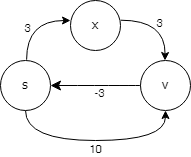
\includegraphics[width=\textwidth]{GrafoPesato01} 
		\caption{Albero di Riccorenza}
	\end{subfigure}
\end{figure} 

Ogni nodo ha due valori:
\begin{itemize}
    \item Dimensione input
    \item Costo locale
\end{itemize}
Ad ogni chiamata sia l'input che il costo vanno a dimezzarsi fino ad arrivare alla foglia che sarà il caso base.

\begin{center}
    \begin{tabular}{||c c||} 
     \hline
     Livello & Contributo \\ [0.5ex] 
     \hline\hline
     0 & n  \\ 
     \hline
     1 & $2*\frac{n}{2} = n$  \\
     \hline
     2 & $4*\frac{n}{4} = n$  \\
     \hline
     \vdots & \vdots \\
     \hline
     i & $2^i*\frac{n}{2^i} = n$ \\ [1ex] 
     \hline
    \end{tabular}
\end{center}



Se andiamo a sommare tutti i contributi di ogni livello dell'albero appena creato avremo che danno tutti lo stesso valore $n$. Grazie a ciò possiamo creare una sommatoria:
$$ T_{MS}(n)=\sum_{i=0}^{?} n$$

Come noteremo la sommatoria dovremmo farla sull'altezza dell'albero, cioè fino a quando l'albero delle chiamate ricorsive arriva al caso base. Sappiamo però che quando incontriamo una foglia, allora allo stesso livello tutte le altre chiamate saranno foglie.\smallskip

Dunque andremo a definire $i$ la nostra altezza incognita.\smallskip

Raccogliamo le informazioni che abbiamo fin ora:

%immagine

Man mano che ci addentriamo nell'albero, la grandezza dell'input diminuisce equamente, e all'ultimo livello avrà formula: $\frac{n}{2^i}$. Però sappiamo che all'ultimo livello, essendo foglia, avremo che la dimensione dell'input e quindi della complessità sarà \textbf{1}.\smallskip

Potremmo quindi impostare un'equazione cosi espressa:

$$\frac{n}{2^i} = 1 \Rightarrow n = 2^i \Rightarrow \log_2 n = \log_2 2^i \Rightarrow \log_2 n = i$$\smallskip

Abbiamo quindi trovato la dimensione di $i$, possiamo quindi sostituirla al punto interrogativo. 

$$ T_{MS}(n)=\sum_{i=0}^{\log_2 n} n \Rightarrow n(\log_2 n+1) = \theta(n\log_2 n)$$
Possiamo dunque approssimare la complessità computazionale di questa equazione di ricorrenza a un caso $n\log_2 n$. 
\smallskip

In questo caso è stato semplice arrivare alla soluzione poichè il valore dell'input fornito ad ogni chiamata ricorsiva è sempre lo stesso e non cambia nel tempo. Potremmo dunque provare a fare un altro esempio andando a cambiare la quantità di chiamate ricorsive ad ogni nodo.

\smallskip

\subsubsection{Esempio 1 con Equazione modificata}

$$T_{MS}(n)= \left\{ \begin{array}{rcl}
    \theta(1) &  n\le1\\
    2 \cdot T(\frac{n}{2})+n^2 & n>1
    \end{array}\right.$$
\smallskip

Andiamo sempre a ragionare come nell'equazione di sopra.

%immagine di valentina che le fa meglio

Come vedremo per ogni livello ora il contributo locale non è piu $n$, ma $n^2$.

In tal senso andiamo a osservare quanto costa ogni livello.

%immagine del costo (tablla)

$$T(n) = \sum_{i=0}^{\log_2 n} \frac{n^2}{2^i} = n^2\sum_{i=0}^{\log_2 n} (\frac{1}{2})^i = n^2 \cdot \theta(1) = \theta(n^2)$$

Il motivo per cui abbiam approssimato a $\theta(1)$ è grazie alla dimostrazione che abbiamo effettuato nelle scorse lezioni.
\subsection{Quicksort}
Il quicksort è un'altro algoritmo di sorting, considerato il miglior algoritmo di ordinamento data la complessità: $\theta(n\lg n)$. Come analizzeremo più avanti questo algoritmo non sarà sempre conveniente, anzi avrà un caso particolare che lo renderà molto sfavorevole $\theta(n^2)$.\medskip

La complessità dell'algoritmo non dipende dalla dimensione di input, ma come viene presentato dall'input stesso.\smallskip

Questo algoritmo sfrutta sempre lo stesso concetto dell'heapsort dividere l'array in 2 parti. La differenza è che gli elementi vengono ordinati dal minore al maggiore, già alla suddivisione dell'array, così da avere due semiarray ordinati già.\bigskip

%%immagine di Valentina dell'array diviso a metà

Concettualmente dobbiamo creare una funzione che ci distribuisce gli elmenti minori di un pre-determinato \textbf{pivot}, un valore dell'array preso per confrontare tutti gli altri elementi. Quel valore sarà un valore di divisione dei due sottovettori.\medskip

Questi confronti devono produrre, dopo già il primo passaggio:
\begin{itemize}
    \item 2 Sequenze non vuote.
    \item Tutti i valori di sinistra sono minori dei valori di destra.
\end{itemize}

\begin{lstlisting}[language=Java]
    QS(A,p,r)
        If p<r then
            q=Partiziona(A,p,r)
            QS(A,p,q)
            QS(A,q+1,r)
\end{lstlisting}

\subsubsection{Requisiti e Ragionamento dietro Partiziona}
\begin{itemize}
    \item $p\le q < r$ che sta a indicare che le partizioni non siano vuote e che gli indici siano distinti di almeno un elemento all'interno dell'array.
    \item $\forall p\le i \le q, \forall q+1 \le j \le r, A[i]\le A[j]$. Questo sta a indicare che per ogni elemento all'interno della sottosequenza di sinistra (i) deve essere minore di ogni elemento della sottosequenza di destra(j).
\end{itemize}
Una volta stabilite e rispettate queste regole possiamo procedere nel ragionamento alla base del quicksort.
\subsubsection{Ragionamento alla base di partiziona}
Utilizzerò 2 indici che farò partire rispettivamente all'inizio e alla fine dell'array. Sceglierò un elemento pivot dell'array, che solitamente è il primo elemento della lista. Dunque inizierò iterativamente a far scorrere i due array, confrontando l'elemento in scorrimento con l'elemento pivot. Di seguito verrà fornito il codice di spiegazione dell'algoritmo per capire cosa fa meglio.

\begin{lstlisting}[language=java]
    Partiziona(A,p,r)
        i=p-1
        j=r+1
        x=A[p]
        Repeat //che sta ad indicare una specie di do while
            Repeat
                j=j-1
            Until A[j]<=y
            Repeat
                i=i+1
            Until A[i]>=x
            If i<j then
                Swap(A[i],A[j])
        Until i>=j
        Return j
\end{lstlisting}

Dunque andremo a confrontare e scambiare gli elementi dell'array che non rispettano la condizione da loro data.

Come detto nel capitolo precedente questo algoritmo deve rispettare la condizione di $p\le j < r$. Proviamo che questo algoritmo non funzioni quindi andiamo a dimostrare per assurdo che questo algoritmo termini violando le due disequazioni:
\begin{itemize}
    \item $p\le r$
    \item $j < r$
\end{itemize}

Assumiamo in partenza che $p<r$, l'algoritmo Partiziona ha appena finito di lavorare e ritorniamo j.

\paragraph{Caso 1}
Per assurdo poniamo $j\ge r$, quindi la nostra relazione sarebbe che $p\le j \le r \Rightarrow j=r$. Poichè noi inizializziamo j allo stesso valore di r (che inizialmente è uguale a $r+1$), e l'algoritmo fa almeno una volta un decremento di r, j sarà uguale a r. E da lì (se il nostro algoritmo farà il return di quella posizione), non dovrebbe muoversi più per rispettare la nostra ipotesi.\smallskip

Dunque i, dall'altra parte confronterà con il primo elemento dell'array, che corrisponde al pivot (x). A questo punto dunque il secondo indice si ferma. Un nuovo ciclo di del repeat esterno partirà e j decrementerà. Ma decrementando andremo a rompere la nostra condizione iniziale, facendo venire la $j<r$.

\paragraph{Caso 2}
Poniamo per assurdo che $j<p$. Questo Vuol dire che potrebbe esistere un valore minore del pivot che si trova in posizione p, ma p o è \textbf{x} o è stato scambiato quindi sarà minore.

\subsubsection{Analisi Asintotica del tempo di esecuzione}

Alla fine della chiamata a Partiziona, possiamo ritrovarci in 2 casi:
%foto parallele dei due casi
\smallskip

In entrambi i casi abbiamo al più $n+1$ incrementi di $i$ e $j$ dal loro inizio (Caso dove j supera i). Mentre in entrambi i casi abbiamo al massimo $\frac{n}{2}$ scambi.

Da ciò possiamo dedurre che abbiamo un $\theta(n)$ di complessità. 
$$T_p(n) = \theta(n)$$

\subsubsection{Analisi della complessità di QuickSort}

Quicksort  effettua una chiamata a partizione dunque già avremo la complessità data dalla funzione $\theta(n)$, poi effettua due chiamate ricorsive di seguito. Da ciò possiamo andare a creare un'equazione di ricorrenza date le chiamate ricorsive a catena.

$$T_{QS}(n) = \left\{ \begin{array}{rcl}
    1 &\mbox{per} & n\le 1\\
    T_{QS}(?) + T_{QS}(?) + \theta(n) & \mbox{se} & n>1
    \end{array}\right.$$

Come potremmo notare non sappiamo a priori (come nel mergesort) le dimensioni dei sottoarray che vengono mandati in chiamata.\smallskip

Possiamo dunuqe riassumere in $q$ una dimensione parametrizzata della chiamata che andremo a sostituire ai punti interrogativi.\smallskip
$$T_{QS}(n) = \left\{ \begin{array}{rcl}
    1 &\mbox{per} & n\le 1\\
    T_{QS}(q) + T_{QS}(n-q) + \theta(n) & \mbox{se} & n>1
    \end{array}\right.$$
Questa q sarà fondamentale nel calcolo della complessità dell'algoritmo. Ovviamente non sappiamo risolvere un'equazione di ricorrenza parametrica, ma a seconda della dimensione di q potremmo farci delle idee sulla complessità dell'algoritmo.\medskip

Infatti a seconda della grandezza di q, potremmo trovarci in un \textbf{caso peggiore}, \textbf{caso migliore} o \textbf{caso medio}.

\paragraph{Caso Peggiore}
Il caso paggiore viene identificato quando abbiamo un grandissimo sbilanciamento nell'albero di ricorrenza. Lo sbilanciamento più grande che un albero può avere è quando $q=1$, cioè il sottoalbero di sinistra sarà sempre il caso base (1).\smallskip

Questo sottoalbero sarà degenere verso destra e diminuirà la sua dimensione molto lentamente (di una grandezza a livello).

%foto della complessità di ogni livello di valentina

\medskip
Come potremmo notare la complessità di questo tipo di albero sarà dato dalla sommatoria di :
$$n+\sum_{i=1}^{n}(n-i+1) = n + \frac{n(n-1)}{2} = \theta(n^2)$$

La complessità di questo caso è quadratica, una complessità molto diversa da quello che ci saremmo aspettati da un quicksort.

\paragraph{Caso Partizioni Uguali}
Il caso in cui Partiziona riesce sempre a dividere l'array in due parti è letteralmente di complessità uguale al mergeSort.

$$T_{QS}(n) = \left\{ \begin{array}{rcl}
    1 &\mbox{per} & n\le 1\\
    T_{QS}(\frac{n}{2}) + T_{QS}(\frac{n}{2}) + \theta(n) & \mbox{se} & n>1
    \end{array}\right.$$

Dunque la complessità computazione è la stessa del merge sort:\smallskip

$$T_{QS}(n) = \theta(n\log_2 n)$$

\subsubsection{Una piccola osservazione (Inutile?)}
Osserviamo questo statement: 
$$\log_2 n = \theta(\log_3 n)$$

questo perchè: $c_1\log_3 n \le \log_2 n \le c_2 \log_3 n$

Per proprietà dei logaritmi possiamo scriver che:
\begin{itemize}
    \item Proprietà 1:$\log_a b = \frac{1}{\log_b a}$
    \item Proprietà 2:$\log_2 n = \frac{\log_3 n}{\log_3 2} = \log_3 n \cdot \log_2 3$
\end{itemize}

Tutto sto ragionamento per dirci alla fine che asintoticamente un logaritmo di qualsiasi base avrà sempre la stessa complessità computazionale di $\theta(\log_3 n)$.

\subsubsection{proprietà degli alberi di ricorrenza del Quicksort}

Vogliamo dimostrre questa formula:
$$n = 2f - 1$$ dove $f$ è il numero di foglie.

\paragraph{Proviamo a dimostrarlo - Per induzione}

La dimostrazione avviene sull'altezza dell'albero ($h$).

\paragraph{Caso Base - Base d'induzione}

$h = 0$ Allora avremmo un solo nodo nell'albero.
$n = 1$, $f = 1 \Rightarrow 1 = 2 * 1 - 1$ Verificato.

\paragraph{Caso induttivo - Passo Induttivo}

$h>0$ In questo caso allora il nodo radice avrà due sottoalberi (x, y) che avranno rispettivamente ($f_x, f_y$) di foglie.\smallskip

Vogliamo allora dimostrare che valga questa proprietà per tutta l'altezza h, ma per farlo dobbiamo dimostrarlo che vale per $h -1$. Sottoalberi non vuoti della nostra ipotesi ci possono essere utili.

Per ipotesi induttiva allora abbiamo che la nostra formula vale fino ad $h-1$:

$$n_x = 2f_x -1$$
$$n_y = 2f_y -1$$

Quindi per farlo valere anche per $h$ dobbiamo:

$$n = 1 + n_x + n_y = 1 + 2f_x -1 + 2f_y -1 = 2(f_x+f_y)-1 = 2f -1$$ Verificato.\medskip

Questa proprietà varrà sia per gli alberi completi che per quelli sbilanciati.

Nei pieni ad esempio avremo un numero di nodi che conosciamo $2^{h+1}$:\smallskip

$n = 2^{h+1} - 1 = 2\cdot 2^h -1$
$f = 2^h$ negli alberi pieni, dunque è verificato.




